\section[Lehramtsstudium (2-Fach-Bachelor) für Gymnasien \& Gesamtschulen bzw. Berufskollegs]{Lehramtsstudium (2-Fach-Bachelor) für Gymnasien \& Gesamtschulen bzw. Berufskollegs}

\begin{multicols*}{2}
An dieser Stelle soll der Ablauf des 2-Fach-Bachelors kurz erläutert werden. Dieser beinhaltet neben dem Fach Physik auch noch weitere Elemente wie euer Zweitfach und die Bildungswissenschaften.
\subsection*{Module}
Innerhalb des Studiums werden Vorlesungen, Übungen und Seminare in Modulen zusammengefasst, die dann in Modulabschlussprüfungen abgeschlossen werden. In den ersten drei Semestern finden die Modulabschlussprüfungen als schriftliche Klausuren statt, danach sind es vor allem mündliche Prüfungen. Die Noten dieser Prüfungen gehen alle in eure spätere Endnote mit ein. Eine Ausnahme stellen die Klausuren in Physik 1 und 2 dar, hier zählt nur die bessere der beiden Noten. Voraussetzung ist dabei selbstverständlich das Bestehen beider Module. Außerdem ist es leider nicht möglich die Modulabschlussprüfungen beliebig oft zu wiederholen. In den Klausuren in Physik 1 bis 3 gibt es vier Versuche und in allen weiteren nur drei.
\subsection*{Die Grundmodule}
In den ersten drei Semestern belegt ihr die grundlegenden Module für das Physikstudium: Dynamik der Teilchen und Teilchensysteme (Physik 1), Thermodynamik und Elektromagnetismus (Physik 2) und Wellen und Quanten (Physik 3). Die Module decken sich im Prinzip mit denen der 1-Fach-Bachelor (1FB) und bestehen aus drei Vorlesungsterminen und zwei (für Physik 1) bzw. einem (Physik 2 \& 3) Übungstermin pro Woche. In der Übung müsst ihr wöchentlich Aufgaben zum Stoff der Vorlesung lösen und insgesamt die Hälfte der Punkte erreichen, um zur abschließenden Klausur zugelassen zu werden. Die Klausur orientiert sich dann ebenfalls an den Inhalten der Übungsaufgaben. Im Unterschied zum 1FB gibt es für euch in Physik 1 noch ein spezielles Mathetutorium. Dieses besteht aus einem verpflichtenden, aber unbenoteten, Test zu Beginn des Semesters und einem wöchentlichen, freiwilligen Tutorium, welches allerdings sehr hilfreich für die Übungen ist. In Physik 2 und Physik 3 hören die 1-Fach-Bachelor zusätzlich noch Theoretische Ergänzungen (TE), die ihr nicht belegen müsst.\\
Im dritten und vierten Semester muss außerdem noch das Modul Experimentelle Übungen, manchmal auch Grundpraktikum genannt, absolviert werden. Innerhalb dieses Moduls werdet ihr alle zwei Wochen eigene Experimente durchführen und diese in Versuchsberichten auswerten, die bewertet werden und eure Modulnote ergeben.
\subsection*{Weitere Module}
Nach den genannten grundlegenden Modulen folgt im vierten Semester das Modul Atom- und Quantenphysik. Dieses ist mit Vorlesung und Übung genauso aufgebaut wie in den vorherigen Semestern, die Modulabschlussprüfung wird allerdings zum ersten Mal als mündliche Prüfung von circa 30-45 Minuten Länge stattfinden.\\
Das fünfte Semester widmet sich dem Modul Struktur der Materie. Es beinhaltet Vorlesungen in Kern- und Teilchenphysik, Physik der kondensierten Materie sowie Astrophysik und Kosmologie. Allerdings müssen nur in den ersten beiden Teilvorlesungen Übungen besucht werden. Auch dieses Modul wird durch eine mündliche Prüfung abgeschlossen.\\
Im sechsten Semester wird das Modul Messtechnik und Signalverarbeitung eingeführt. Hier müsst ihr die Kombination aus Vorlesung und Übung in den Grundlagen der Signalverarbeitung absolvieren und durch eine mündliche Prüfung abschließen.\\
Des Weiteren wird in den Semestern fünf und sechs das Modul Grundlagen der Fachdidaktik und Erkenntnistheorie absolviert. Es beinhaltet eine Vorlesung zur Einführung in die Fachdidaktik der Physik für das Lehramt Physik mit abschließender mündlichen Prüfung und ein Seminar zur Theorie, Geschichte und Kultur der Naturwissenschaften, in dem ihr eine Seminararbeit, meistens ein Referat, erstellen müsst, welches nicht benotet wird.\\
Am Ende könnt ihr euch noch entscheiden, ob ihr eure Bachelorarbeit in der Physik oder in einem eurer anderen Fächer schreiben möchtet.\\
Genauere Informationen zu den Inhalten und Prüfungsleistungen der Module, sowie einen beispielhaften Studienverlaufsplan findet ihr auf der Homepage des Fachbereichs (\url{https://www.uni-muenster.de/Physik}) und in eurer jeweiligen Prüfungsordnung (diese gibt es auch auf der Homepage).
\end{multicols*}

% \newpage

\begin{minipage}{\textwidth}
\begin{multicols*}{2}
\begin{wraptable}[31]{r}{2cm}
        \centering
        \begin{tabular}{|c|c|c|}
        \hline
        \multirow{2}{*}{\textbf{Semester}} & \multicolumn{2}{c|}{\multirow{2}{*}{\textbf{Module im 2-Fach-Bachelor Physik}}} \\ 
        & \multicolumn{2}{c|}{} \\
        \hline
        \multirow{3}{1cm}{1. (WiSe)} & \multirow{3}{3cm}{\makecell{Physik~I\\ \footnotesize 15~LP}} & \\
        &&\\
        &&\\
        \cline{1-2}
        \multirow{3}{1cm}{2. (SoSe)} & \multirow{3}{3cm}{\makecell{Physik~II \\ \footnotesize 10~LP}} & \\
        &&\\
        &&\\
        \hline
        \multirow{3}{1cm}{3. (WiSe)} & \multirow{3}{3cm}{\makecell{Physik~III \\ \footnotesize 10~LP}} & \multirow{7}{3cm}{\makecell{Experimentelle\\Übungen~I \\ \footnotesize 6~LP}} \\ 
        &&\\
        &&\\
        \cline{1-2}
        \multirow{4}{1cm}{4. (SoSe)} & \multirow{4}{3cm}{\makecell{Atom- und \\Quantenphysik \\ \footnotesize 10~LP}} & \\
        &&\\
        &&\\
        &&\\
        \hline
        \multirow{4}{1cm}{5. (WiSe)} & \multirow{4}{3.2cm}{\makecell{Struktur der\\ Materie \\ \footnotesize 12~LP}} & \multirow{8}{3cm}{\makecell{Grundlagen der\\Fachdidaktik und \\Erkenntnistheorie\\\footnotesize 4~LP}} \\
        &&\\
        &&\\
        &&\\
        \cline{1-2}
        \multirow{7}{1cm}{6. (SoSe)} & \multirow{4}{3.5cm}{\makecell{Messtechnik und\\Signalverarbeitung \\ \footnotesize 8~LP}} & \\
        &&\\
        &&\\
        &&\\
        \cline{3-3}
        & \multirow{3}{3cm}{\makecell{Bachelorarbeit \\ \footnotesize 10~LP~(WPM)}} &\\
        &&\\
        &&\\
        \hline
    \end{tabular}
    %\label{Tab.2FB_Module}
\end{wraptable}

\subsection*{Bildungswissenschaften}
In den Bildungswissenschaften müsst ihr drei Pflichtmodule absolvieren, die namentlich zwar nach Lehramt für Gymnasien/Gesamtschulen (Gym/Ge) sowie Berufskolleg (BK) aufgeteilt sind, sich strukturell aber sehr ähneln. Zunächst muss das Modul Einführung in Grundfragen von Erziehung, Bildung und Schule (für Gym/Ge) bzw. Einführung in Grundfragen beruflicher Bildung (für BK) absolviert werden. Dazu gehören eine Vorlesung inklusive Tutorium und abschließender Klausur sowie ein frei wählbares Seminar mit eigener Prüfungsleistung. Dieses Modul sollte im ersten oder zweiten Semester belegt werden, wobei sich meistens das zweite Semester besser eignet. Außerdem müssen noch zwei Praktika während des Bachelors absolviert werden. Zunächst das Eignungs- und Orientierungspraktikum (EOP), in welchem ihr fünf Wochen in einer von euch gewählten schulischen Einrichtung (passend zu eurer angestrebten Schulform) hospitiert und später das Berufsfeldpraktikum (BFP) über 4 Wochen, in dem ihr Berufsmöglichkeiten außerhalb des Lehramts kennen lernen sollt.  Dazu gibt es jeweils ein vorbereitendes Seminar (gegebenenfalls auch begleitend oder nachbereitend) und ihr müsst einen Praktikumsbericht anfertigen. Dieser ist im EOP benotet und im BFP unbenotet.\\
Weitere Informationen zu den Modulen sowie die Prüfungsordnung findet ihr auf den Seiten der Bildungswissenschaften (\url{https://www.uni-muenster.de/Bildungswissenschaften/}).\\ 
Das sind zunächst die wichtigsten Informationen, die ihr für die Bewältigung eures Bachelorstudiums braucht. Solltet ihr noch weitere Fragen haben, könnt ihr gerne in der Fachschaft vorbei schauen! Bei grundlegenden Fragen könnt ihr auch zur Zentralen Studienberatung gehen. Außerdem empfiehlt es sich natürlich, die speziellen Infoveranstaltungen für 2-Fach-Bachelor während der Orientierungswoche zu besuchen. :-) 

\columnbreak
\vfill
\hfill

\end{multicols*}
\end{minipage}

\begin{multicols}{2}

\mbox{}
\vspace{5ex}
\fibelsig{Andrea, Moritz}
\columnbreak

\begin{tikzpicture}[remember picture,overlay,shift={(current page.south east)}]
\node[anchor=south east,xshift=-1.4cm,yshift=2.1cm]{
	\fibelimgtext{
		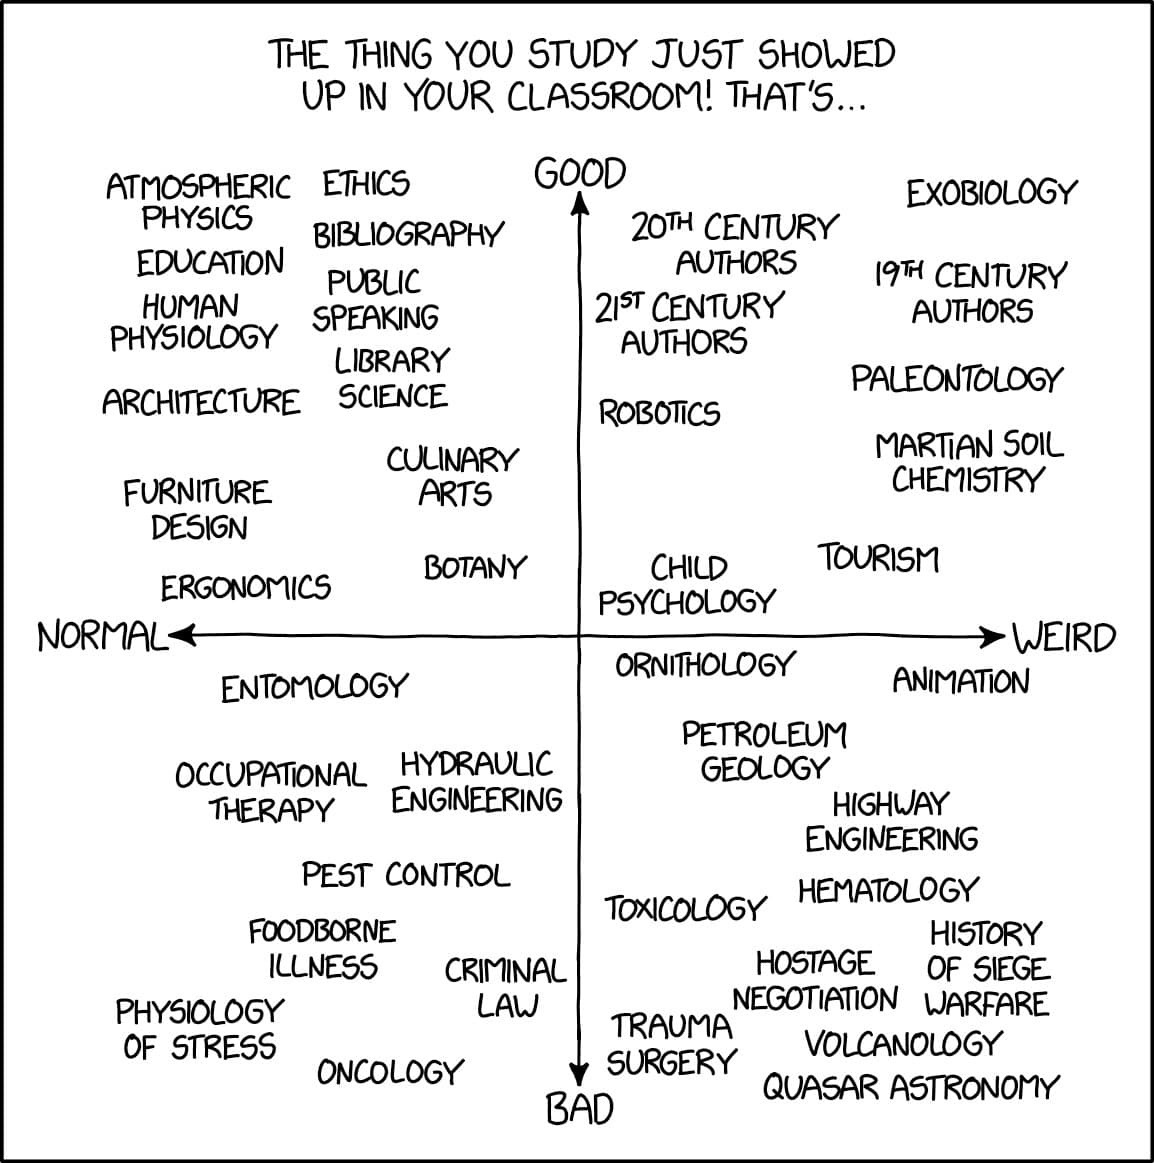
\includegraphics[width=.9\columnwidth]{res/xkcd/xkcd_lehramt.jpg}
	}{\url{https://xkcd.com/2466}}
    };
\end{tikzpicture}
\begin{center}
\end{center}

%\begin{center}
%	\fibelimgtext{
%		\includegraphics[width=\columnwidth, height=0.23\textheight]{res/xkcd/894_progeny.png}
%	}{\url{https://xkcd.com/894}}
%\end{center}
\end{multicols}
